\documentclass{article}
\usepackage[utf8]{inputenc}
\usepackage{caption}
\usepackage[margin=1in]{geometry}
\usepackage{graphicx}
\usepackage{pdfpages}
\usepackage{float}
\pdfminorversion=7

\begin{document}
\begin{titlepage}


\centering
\vspace*{2cm}
{\Huge Final Project Report\par}
\vspace{.25cm}
{\LARGE Course Evaluation System\par}
\vspace{1cm}
{\Large Team EVAL\par}
\vspace{.2cm}
{\Large Jovon Craig, Sam Elliott, Yuanqi Guo, Robert Judkins, and Stanley Small\par}
\vspace{1cm}
{\Large Client: Dr. Harlan Onsrud\par}
\vspace{1cm}
{\Large May 7, 2019\par}
\vspace{11cm}

University of Maine - Spring of 2019 - COS 497

Instructor: Professor Terry Yoo

\end{titlepage}

\newpage

\begin{center}
{\includegraphics[scale=.2]{images/team_logo.png}} \\ 	\bigskip
{\LARGE Course Evaluation System } \\ \medskip
{\large Final Project Report } \\ \medskip
\end{center}

\tableofcontents

\newpage

\section{Introduction}

\subsection{Purpose of This Project}

For our capstone project, Team EVAL created the Course Evaluation System, a web application designed to be intuitive and versatile for college instructors. This new system, which will be tested first at the University of Maine, allows one to quickly create course evaluation surveys and review their responses. We undertook this project for our client, Dr. Harlan Onsrud, who wanted a more efficient way to process course evaluations. By making and documenting the software, the team has gained valuable skills in software engineering, programming, and technical writing.

\subsection{Purpose of This Document}

This final project document gives an overview of our course evaluation system, the purpose of it, and why we believe it is useful. We first talk about existing evaluation creation software and how it is not tailored to college instructors and administrators. The next section goes into more detail about the system, discussing its requirements, architecture, development process, and user interface. The last section describes how the finished product improves productivity, our thoughts on what we learned from the project, and the steps we would take to improve the product.

This document is intended for the development team, the product client, and potential users of the system. Team EVAL needs this document to summarize the product's development in job interviews. The client, Professor Harlan Onsrud, also needs it to verify that we designed the system according to his needs. The document helps the software's users by informing them what the system does and how it particularly helps them with their work.

\subsection{References}

Craig, J., Elliott, S., Judkins, R., \& Small, S. 29 October 2018. \textit{System Requirements Specification.}
\vspace{3mm}\newline
Craig, J., Elliott, S., Judkins, R., \& Small, S. 16 November 2018. \textit{System Design Document.}
\vspace{3mm}\newline
Craig, J., Elliott, S., Judkins, R., \& Small, S. 30 November 2018. \textit{User Interface Design Document.}
\vspace{3mm}\newline
Craig, J., Elliott, S., Guo, Y., Judkins, R., \& Small, S. 14 March 2019. \textit{Code Inspection Report.}
\vspace{3mm}\newline
Craig, J., Elliott, S., Guo, Y., Judkins, R., \& Small, S. 4 April 2019. \textit{Administrator Manual.}
\vspace{3mm}\newline
Craig, J., Elliott, S., Guo, Y., Judkins, R., \& Small, S. 18 April 2019. \textit{User Manual.}
\vspace{3mm}\newline
Onsrud, H. ``Example Question Selection Form.'' See Appendix H.
\vspace{3mm}\newline
Onsrud, H. ``Example Results Display.'' See Appendix I.
\vspace{3mm}\newline
LimeSurvey: The online survey tool - open source surveys. (n.d.). Retrieved from

https://www.limesurvey.org/.

\section{Purpose of This System}

\subsection{Our Problem}

In 2015, there were more than 4,600 higher-education institutions in the United States. Virtually all of them offer a breadth of college courses for students to complete and carry them through their academic careers. At the end of a course, students typically fill out an evaluation manually so that teachers know how they are performing in their roles. Unfortunately, many institutions, such as the University of Maine, are behind in the technology that can be used for this task.

The University of Maine has traditionally used Scantron sheets for course evaluation forms. As Team EVAL knows, filling in tiny bubbles with pencil and paper is tedious. It is also hard work for the college administration to use Scantron sheets. They need to scan the forms for every student in every course, and the data then needs to be collected as forms that are readable for instructors. The University of Maine must upgrade its process to keep with the times and exploit today's technology.

\subsection{Existing Survey Software}

Several software solutions currently exist that allow users to create, modify, and publish surveys. One notable example is LimeSurvey, a free and open-source tool that is operated online. The team acknowledges the immense amount of work put into creating LimeSurvey, with its selection of question types, scalability, visualization features, and other powerful functionality. However, LimeSurvey has always been general-purpose software; it is aimed at multiple types of users who want to make surveys. Consequently, it is complex and has a high learning curve.

College teachers and administrators need to jump through hoops to use tools like LimeSurvey, which are not always easy or intuitive. Their evaluations are highly standardized and sent to potentially hundreds of students, yet LimeSurvey and similar software do not account for these qualities. A college instructor would have to manually input every field, question, and class roll into each evaluation from scratch. UMaine is using another service, Blue by Explorance, that has the necessary functionality, but it is expensive to use for a university and often inflexible if administers want to differ from the norm. These are some of the reasons why our client, Dr. Onsrud, wants us to create software that is better suited to instructors. We believe our Course Evaluation System will help instructors make useful surveys efficiently and easily. 

\newpage

\section{About This System}

\subsection{System Requirements}

Near the beginning of the project, we met with Professor Onsrud to solicit the system requirements, what the evaluation system must do to function as Dr. Onsrud intends. The System Requirements Specification (SRS) divides the requirements into two categories. The functional requirements specify the major actions a user can perform with the system. They are listed in Table 1 below:

\begin{center}

\begin{tabular}{|p{1.5cm}|p{1.5cm}|p{3.5cm}|p{6cm}|} 
\hline
\textbf{Number} & \textbf{Priority} & \textbf{Name} & \textbf{Description} \\
\hline
1 & 5 & Log in to system & A user logs in with a Google e-mail address and password \\ 
\hline
2 & 5 & Create evaluation & A user creates a new evaluation form for a class \\ 
\hline
3 & 5 & Edit evaluation & A user enters and edits information and questions for an evaluation form \\  
\hline
4 & 5 & Publish evaluation & A user publishes an evaluation form \\
\hline
5 & 5 & View evaluation results & A user reviews the survey results of a category of courses\\ 
\hline
\end{tabular}
\captionof{table}{Functional requirements}
\end{center}

The non-functional requirements state the system's qualities that do not pertain to how the program behaves. They are listed below in Table 2:

\begin{center}
\begin{tabular}{|p{1.5cm}|p{1.5cm}|p{8cm}|}
\hline
\textbf{Number} & \textbf{Priority} & \textbf{Description} \\
\hline
1 & 3 & The software should be supported by the latest versions of Windows, Mac, Linux, iOS, and Android.\\ 
\hline
2 & 4 & The software should be accessible by the latest versions of Safari, Chrome, Firefox, and Edge.\\ 
\hline
3 & 5 & All questions entered by the teacher or administrator shall appear on the output survey.\\  
\hline
4 & 5 & All data stored in the program's database shall be valid.\\
\hline
5 & 5 & All collected survey data shall not be alterable.\\ 
\hline
6 & 4 & Teachers shall not be able to access data of courses other than their own.\\ 
\hline
7 & 3 & The mean time between failures should be at least 60 minutes.\\ 
\hline
8 & 5 & Students shall have no access to any data stored by the program.\\ 
\hline
9 & 5 & All survey responses (except signed comments) shall be anonymous.\\ 
\hline
10 & 2 & The software should scale to at least three universites, 1000 courses per semester, 1000 teachers per university, and 500 students per course.\\  
\hline
11 & 1 & The software should not exceed 500 MB in size.\\
\hline
12 & 4 & The software's source code shall be open-source and shall use a GPLv2 license.\\ 
\hline
13 & 4 & The licensing requirements of any non-original code shall be met.\\ 
\hline
14 & 4 & The software shall meet UMaine AFUM requirements.\\ 
\hline
\end{tabular}
\captionof{table}{Non-functional requirements}
\end{center}

\subsection{System Architecture}

\begin{center}
\begin{figure}[H]
\centering
\vspace{2mm}
{\includegraphics[scale=.75]{images/component_diagram.png}}
\captionof{figure}{Component diagram of the system}
\end{figure}
\end{center}

Our system features a modular design, with many distinct parts which communicate via an API. The front end implements the user interface, and it is written in JavaScript and the React framework. The back end communicates with the system's databases and is written in Python and the Flask framework. We are using two databases, one maintained by LimeSurvey and another maintained by our system. Additionally, the API will communicate with Google Authentication to authenticate users. The design and implementation of our system can be found in the System Design Document (SDD). The system's components are displayed in Figure 1 above.

By maintaining a modular approach to the design of the system, team members can work independently on separate components of the system. Moreover, by keeping the LimeSurvey codebase separate from our system, we can update our original code without disrupting the functionality of LimeSurvey.

\subsection{Our Process}

As our project required following a strict timeline over the 2018-2019 academic year, Team EVAL used a software development process, which subscribed to both waterfall and agile methodologies. We primarily used the Scrum framework to develop our product. The team held stand-up meetings twice a week, as well as biweekly Scrum planning meetings. We also followed the V-model, a waterfall-like process that emphasizes verification in the first half of development and validation in the second half. A diagram of the V-model is shown as Figure 2 on the next page.

\begin{center}
\begin{figure}[H]
\centering
\vspace{2mm}
{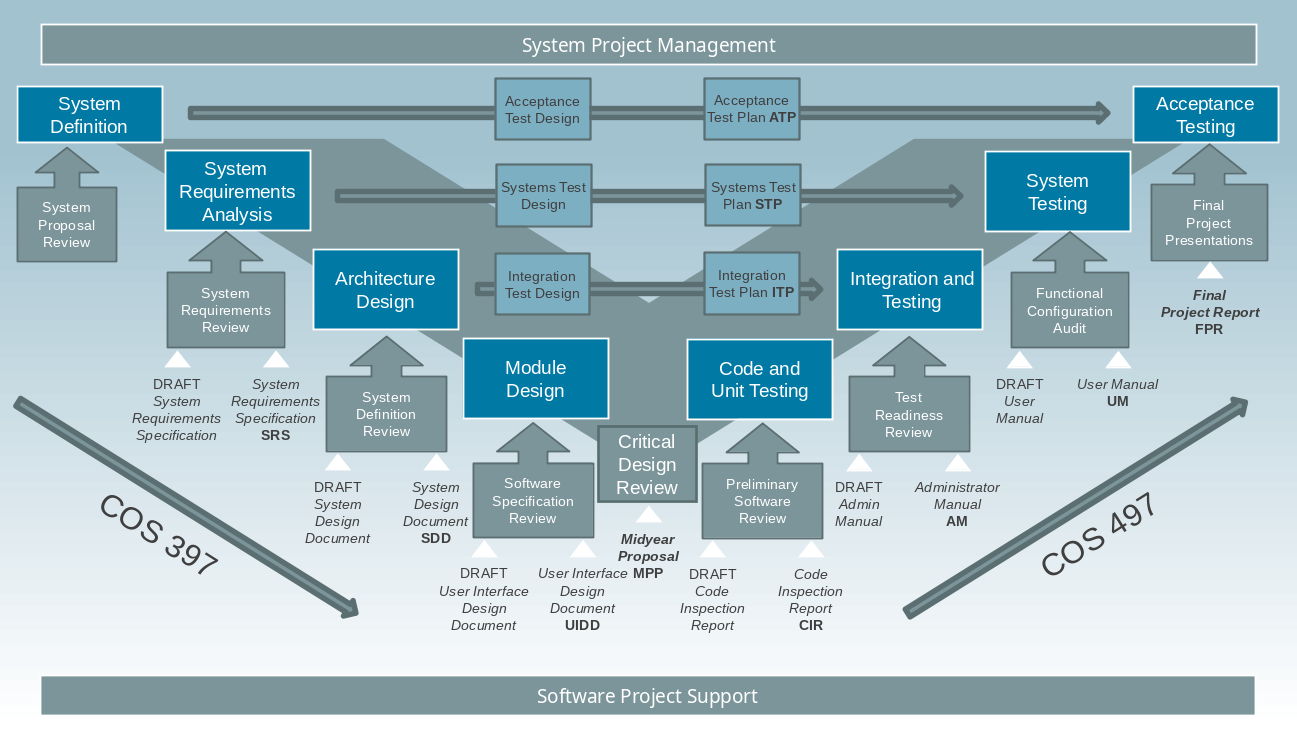
\includegraphics[scale=.6]{images/V-model-Yoo.png}}
\captionof{figure}{The V-model, showing the steps in the process}
\end{figure}
\end{center}

The team took additional measures to organize our development of the system. We assigned team roles according to the Team Software Process: the team leader, the development manager, the planning manager, the process manager, and the support manager. In addition, the team frequently collaborated with the client to ensure the correct product was built. As for tools, Github was used to store and maintain the code, and Docker ensured our code could run in a familiar environment on different machines.

Team EVAL wrote numerous tests over the course of the project to ensure that the course evaluation system met its functional requirements. On the back end, Jovon and Tom wrote several unit tests for each endpoint, both positive and negative, with Python's ``unittest'' library. These tests check whether the routes can handle API calls with a variety of input. Sam wrote additional tests for the front end using Webdriver.io. He included unit tests that validate functions specific to the user interface, such as loading data into text fields, and integration tests that interact with the API to validate whether the UI is properly using our database.

\subsection{User Interface}

The user interface is a pivotal part of the user experience and is important for our product. Our goal of the system was to make an easy-to-use software that allows users to create course evaluations for their classes on a web application. Users have no interaction with the back-end architecture and can only see the user interface, so the ease of use relies entirely on the front-end UI. Detailed descriptions of every aspect of our user interface can be found in the User Interface Design Document (UIDD).

\newpage

The overarching theme for the user interface is "less is more''.  The interface has as few extraneous elements as possible, is as intuitive as possible, and does not require a large amount of effort to understand the system. To this end, all functionality of the product is accessible from the home page, of which a screenshot is shown below as Figure 3.

\begin{center}
\begin{figure}[H]
    \centering
    {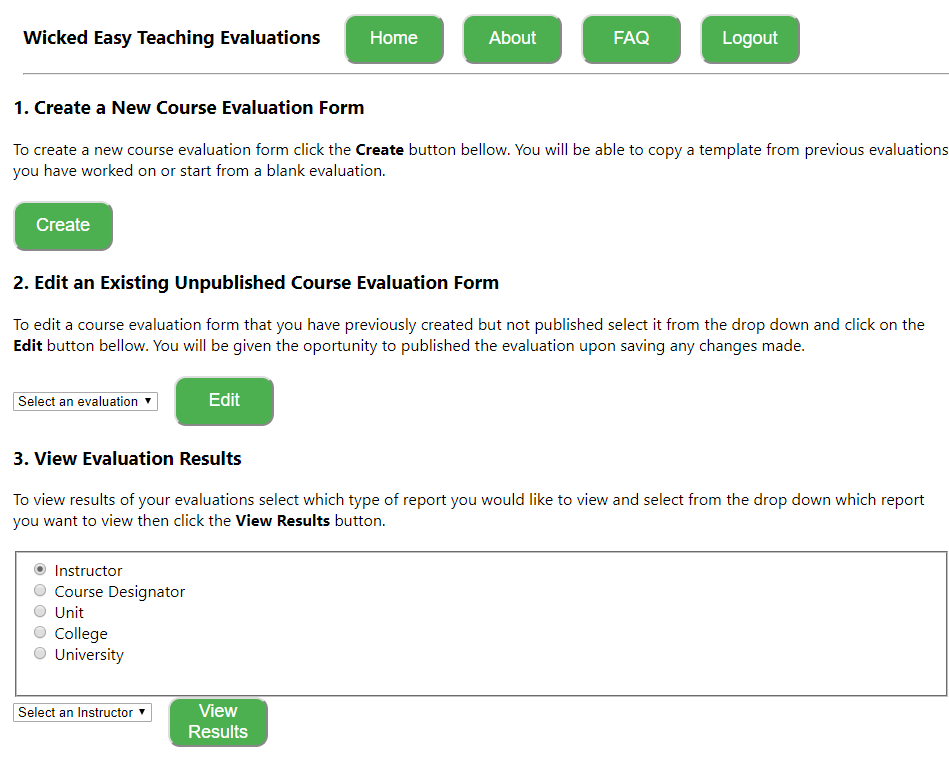
\includegraphics[scale=.6]{images/homeScreen.png}}
    \caption{Home screen of the user interface}
\end{figure}
\end{center}

After passing the landing screen, the user is instantly aware of the functions that one can make through the home screen. The interface allows users to create new evaluations, view their existing and previous evaluations, and view statistics for the results of completed evaluations. Users can also select an existing form as a preset for a new evaluation. To reduce confusion, help text for different features is present on the same page and does not require users to navigate away from it.

\newpage

Our user interface was designed to emulate the physical processes that have been in place at the University of Maine for administering teaching evaluations. This decision was made to make the transition to our software easier for all parties involved. The same information is collected to allow an easy transition for the university to use our product.

\begin{center}
\begin{figure}[H]
  \centering
  {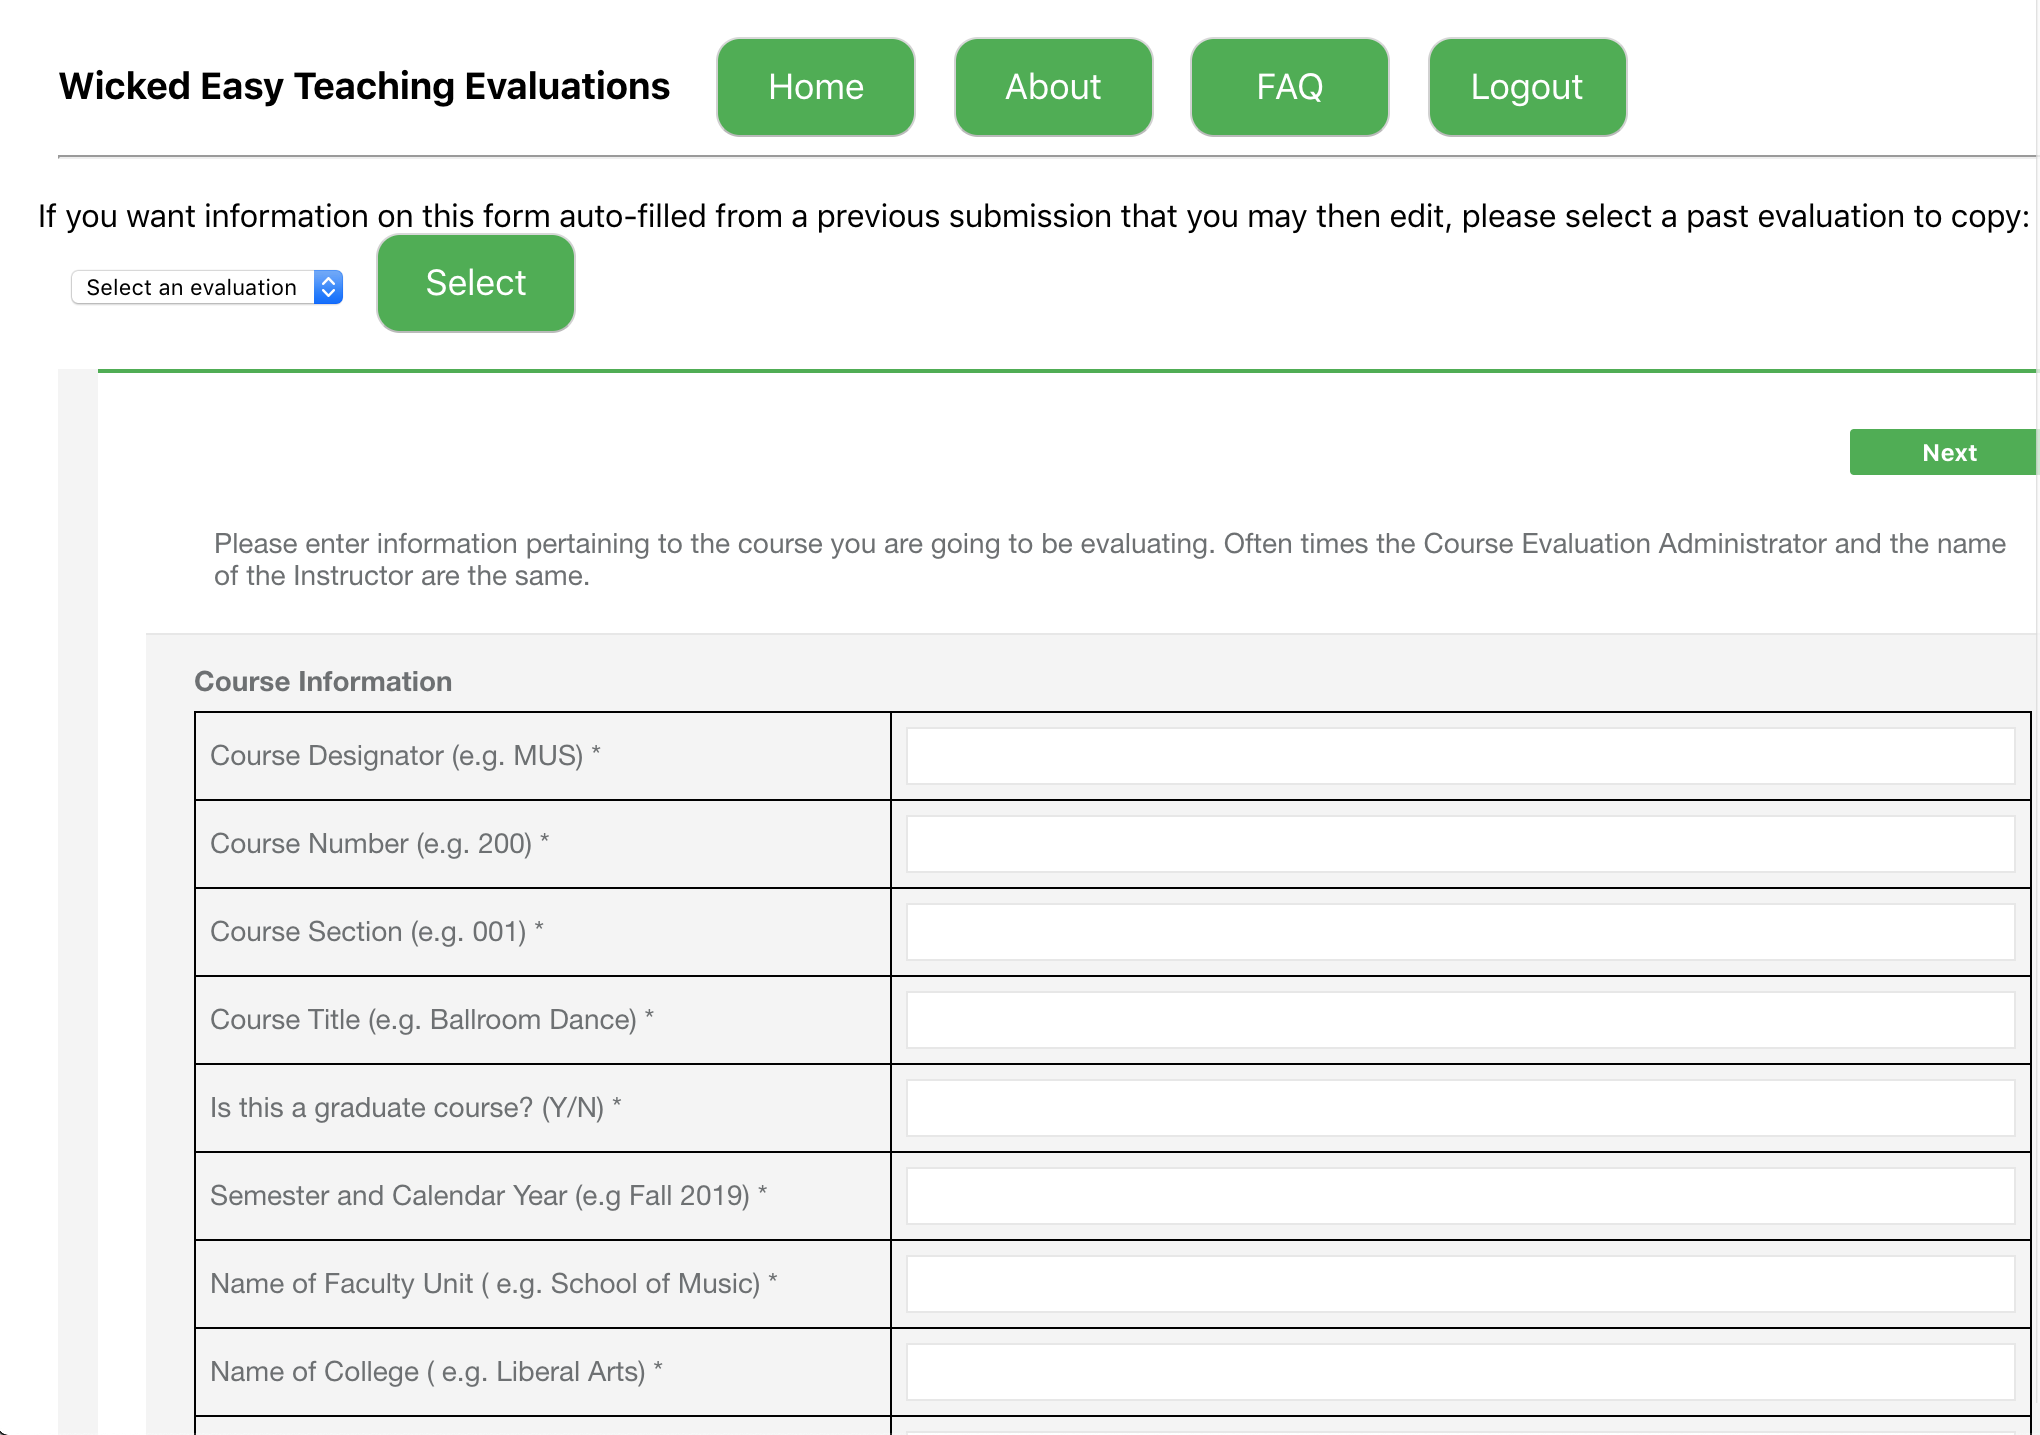
\includegraphics[width=6.2in]{images/final_create_screen.png}}
   \caption{The first screen seen when creating an evaluation}
\end{figure}
\end{center}

Once a user decides to create an evaluation, they are met with a simple screen with several forms for them to fill out. The interface is designed to be self-explanatory so that anyone can create an evaluation with no troubles. The user is presented with three screens to fill out the information about their course, their students, and the questions they would like to include in their evaluation.

Overall, our interface is designed with the hopes that any user could use our product easily and without any hold-ups. They can effortlessly go through the various screens to create, edit, or publish an evaluation and view the results once their students have completed the evaluation.

\newpage

\section{Conclusion}

\subsection{Needs This System Meets}

Our course evaluation system will bring the University of Maine into the modern era of using technology to evaluate courses. Using our software, an instructor can choose questions for their surveys with ease, and students are able to take the surveys anytime and anywhere. It is convenient to publish a survey, as LimeSurvey handles its lifetime and e-mails to its participants. The results are automatically fed back into the software, and the instructor can view statistics of the results and download them afterwards. The administrator no longer needs to manually distribute evaluations, collect them, and scan them, and manually do statistical analysis to get their results. The system does these functions automatically, making the process of evaluations significantly easier for administrators and teachers.

Furthermore, this product eliminates the need for Scantron sheets, saving paper and the need for students to dedicate time in class fill out bubble sheets. It instead provides a fast and simple way to distribute evaluations to all students in a desired course. Lastly, the product meets Dr. Onsrud's most important requirements. It is free and open-source, and it is compatible with all major web browers. All survey responses are anonymous, and the data stored by the program cannot be accessed by students. Eventually, our system will be free to use for instructors at the University of Maine and by any teachers elsewhere.

\subsection{What We Have Learned}

Throughout the process of developing the system, the team learned numerous lessons. Members of the team will attempt to incorporate the values of these lessons into future projects and our professions. 

One of the first lessons learned in the project was the importance of active and effective communication. Any progress made by the team relies on communication and teamwork. Although the team did use Slack to communicate, we should have added the client into the Slack channel to keep the client informed and more active in the project. As the client spent more time away from the project in the second semester, productivity and progress waned.

Another lesson learned was that defining and following a process is important for developing a working and effective product. Without adhering to the process defined by Dr. Yoo, progress would have been greatly diminished. The process allowed the team to ensure that we stayed on task and continued working throughout the course of the project. 

The team also realized that early and constant feedback is essential, especially from the client. As mentioned previously, the inability of the team to effectively communicate with the client during the second semester of the project made it difficult to complete certain functionality to the needs of the client. While process remains important, the ability to always have a working implementation remains key. The team should have worked on creating a minimum viable product (MVP) first, then receiving feedback later. 

Finally, the team learned that software building is not equivalent to coding. As Fred Brooks states, only about one sixth of a team's time should be spent coding. The rest of the time is spent planning and testing, to ensure the team creates the right product. Verification and validation are key components of building software that both the team and the client are happy with. Throughout the process, the team learned that system development depends on much more than just coding. 

\subsection{Future Work}

Despite working on the project for an academic year with five team members, Team EVAL did not achieve everything we set out to accomplish. This section describes the elements and features the team would have liked to include in the system, had time allowed. 

First, the team wishes to improve the appearance and functionality of the user interface. The current version of the project represents the first generation of what can potentially be a very user-friendly product. The team wishes to have groups for testing and evaluating the evaluation system to ensure the system accomplishes all of the goals defined by the client. 

Second, the team would like to expand on results reporting. The results accessible to users of the system remains limited at this point in time. The team wishes to expand the reporting capabilities of the system to provide more advanced statistics representing feedback for instructors, the college, and the schools within the system. 

Additionally, the team would like make the evaluation structure more flexible. Currently, the system is tuned to the needs of the University of Maine's requirements for teaching evaluations. To make the system more usable and accessible to a wider audience, the team would like to provide the opportunity for more customization and personalization of the evaluations to system users. 

Finally, we wish to automate the deletion of data after the semester concludes. As anonymity and security remain some of the key components of the teaching evaluation system, the team would like to discard information that is not currently being used. 

\section{Acknowledgments}

We would like to thank multiple people for giving us the opportunity to work on the Course Evaluation System. We thank Dr. Harlan Onsrud for letting us work on the course evaluation system and being patient with us during the development process. We thank Dr. Terry Yoo for guiding us in our capstone project and teaching us good software engineering practices. We could not have finished the project without Yoo. Finally, we thank the developers of LimeSurvey for providing an open-source survey creation program that we could incorporate into our software, saving us development time.

\newpage
\appendix

\section{Document Contributions}

This section lists the contributions that each member of Team EVAL made to this document.

\medskip

Stanley Small wrote the system architecture section and most of the conclusion, including the ``What We Have Learned'' and ``Future Work'' sections. He also added Figure 4 to the document.

Jovon Craig wrote the system requirements section, ``Needs This System Meets'' section, and most of the introduction, ``Purpose of This System'' section, and process section. He also made revisions to the whole document.

Sam Elliott wrote most of the user interface section and contributed to the testing section. He made some revisions to the document as a whole.

Robert Judkins wrote a part of the user interface section and made a few revisions to the conclusion.

Yuanqi Guo added more content to the ``Existing Survey Software'' section and ``Needs This System Meets'' section. 

\newpage


\includepdf[scale=0.85,pages=1,pagecommand=\section{System Requirements Specification}]{srs.pdf}

\includepdf[scale=0.85,pages=2-]{srs.pdf}

\newpage

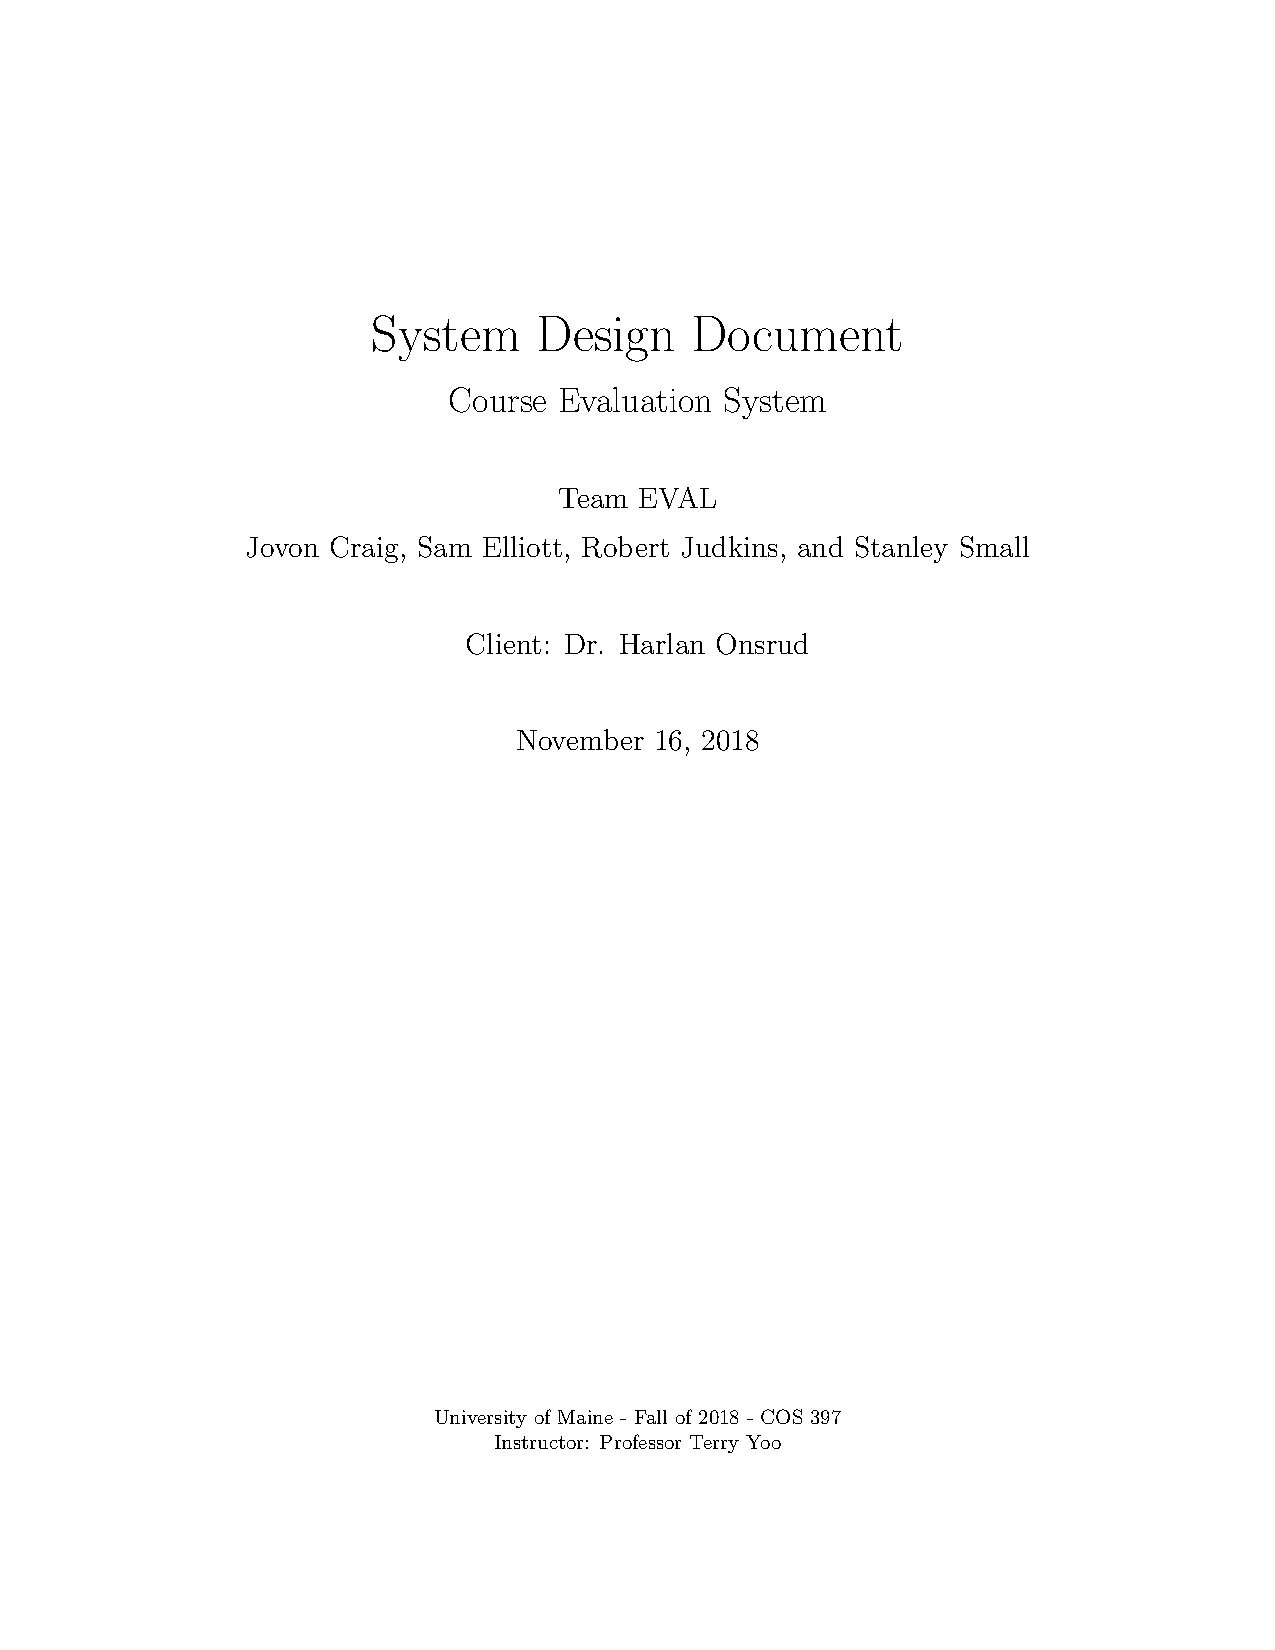
\includepdf[scale=0.85,pages=1,pagecommand=\section{System Design Document}]{sdd.pdf}
\includepdf[scale=0.85,pages=2-]{sdd.pdf}

\newpage

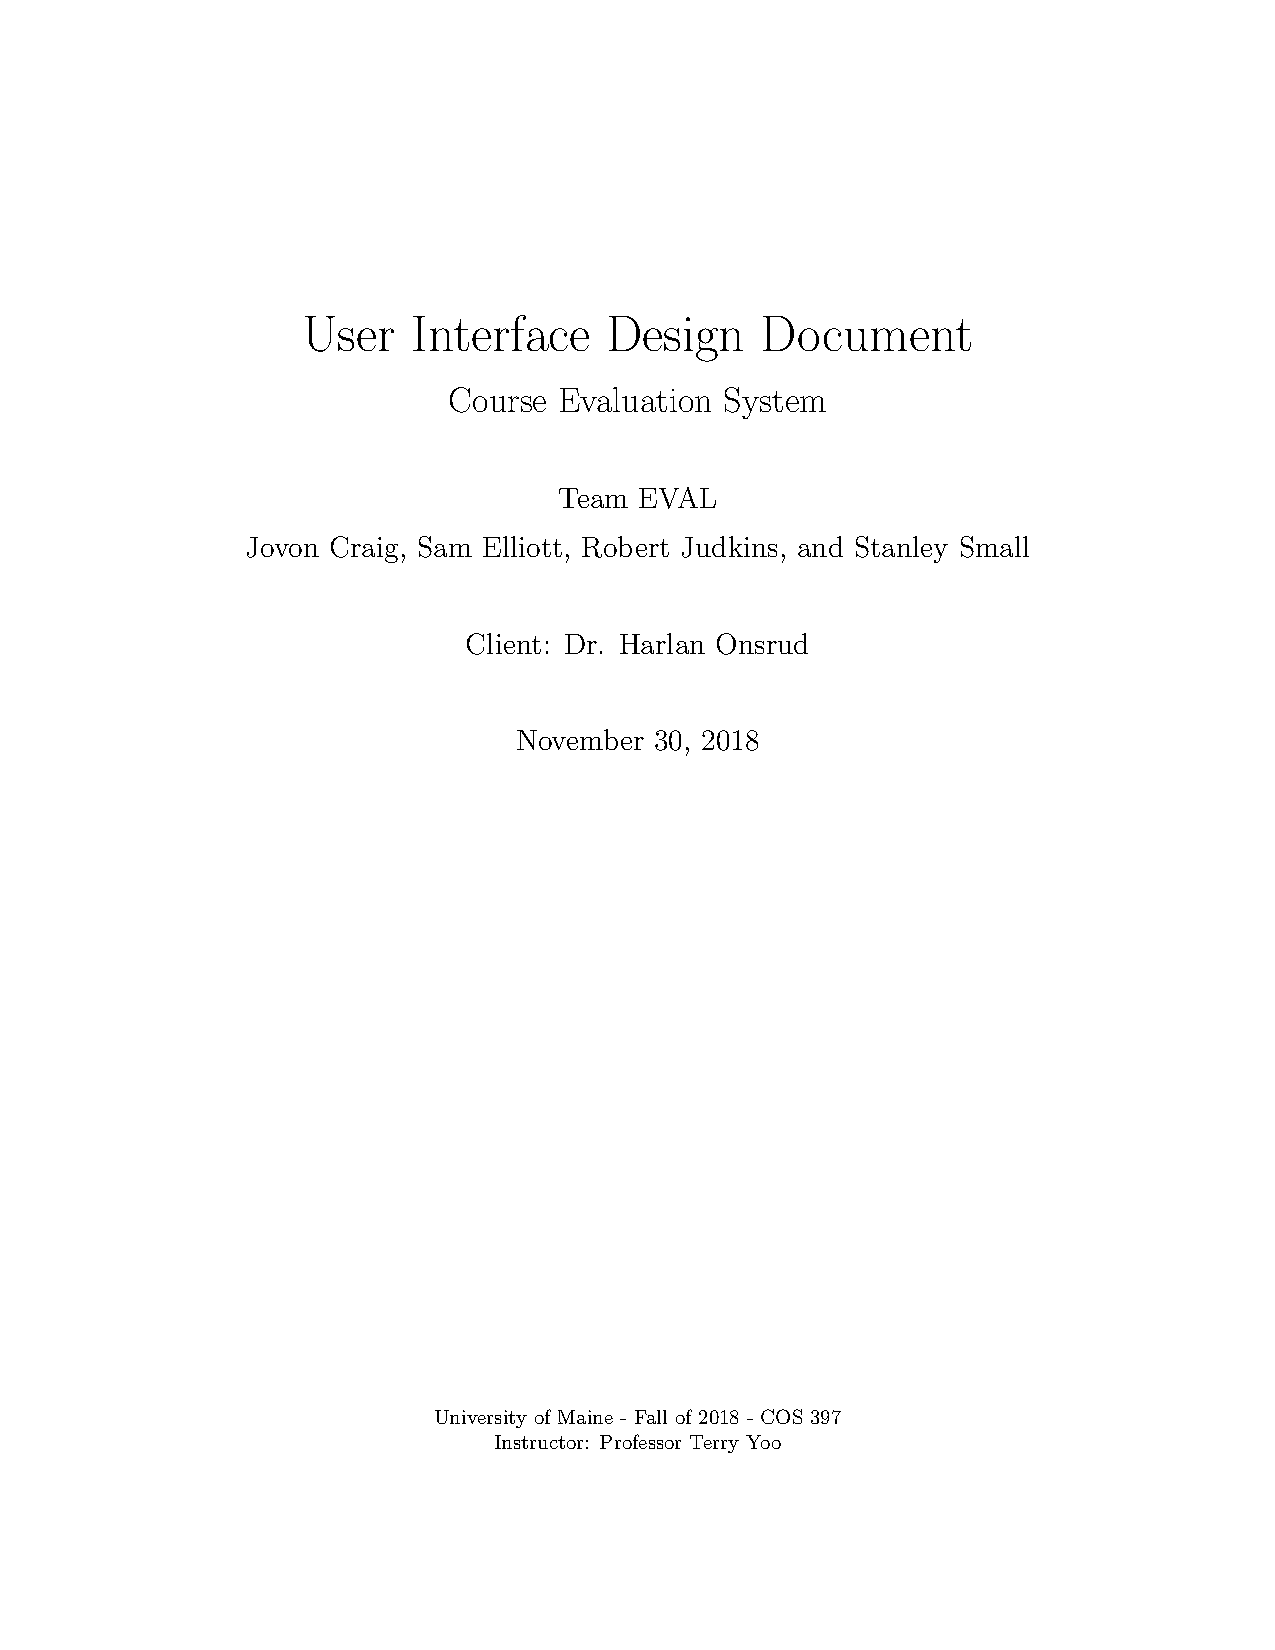
\includepdf[scale=0.85,pages=1,pagecommand=\section{User Interface Design Document}]{uidd.pdf}
\includepdf[scale=0.85,pages=2-]{uidd.pdf}

\newpage

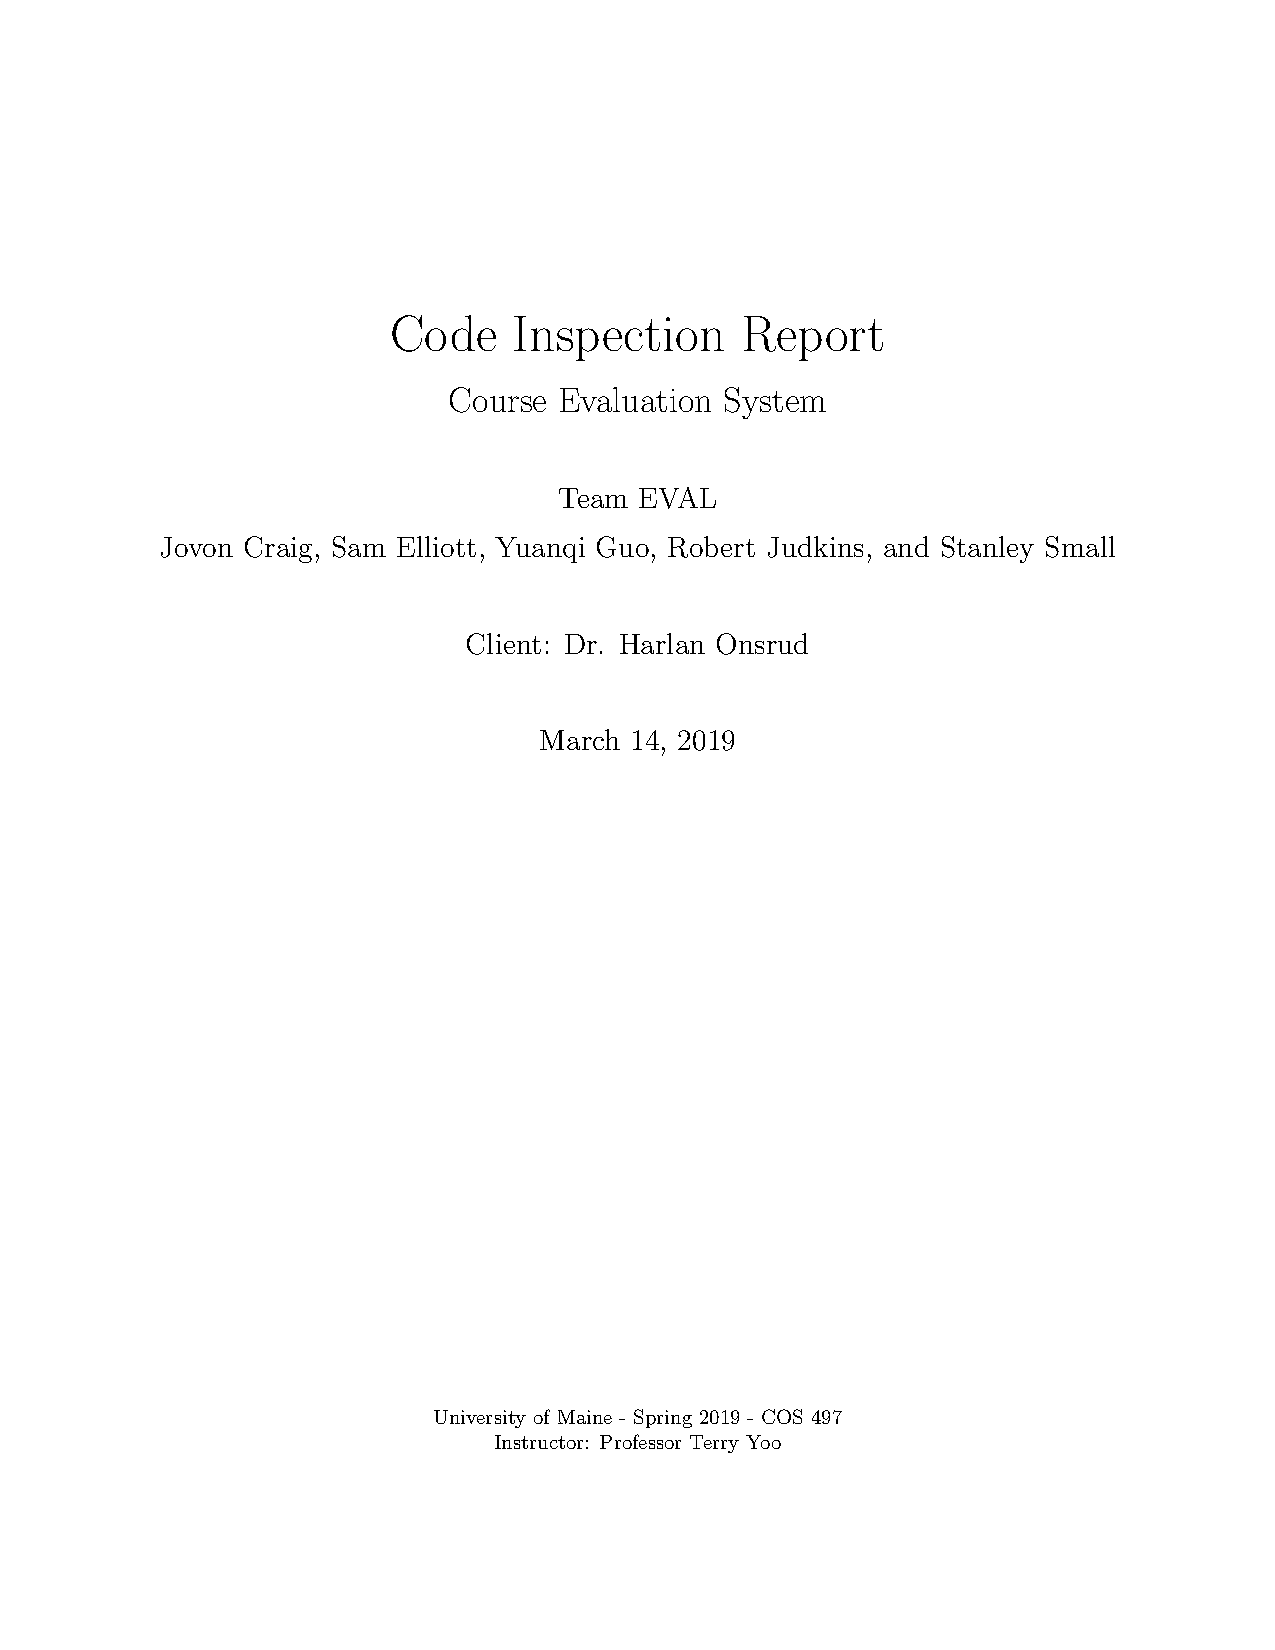
\includepdf[scale=0.85,pages=1,pagecommand=\section{Code Inspection Report}]{cir.pdf}
\includepdf[scale=0.85,pages=2-]{cir.pdf}

\newpage

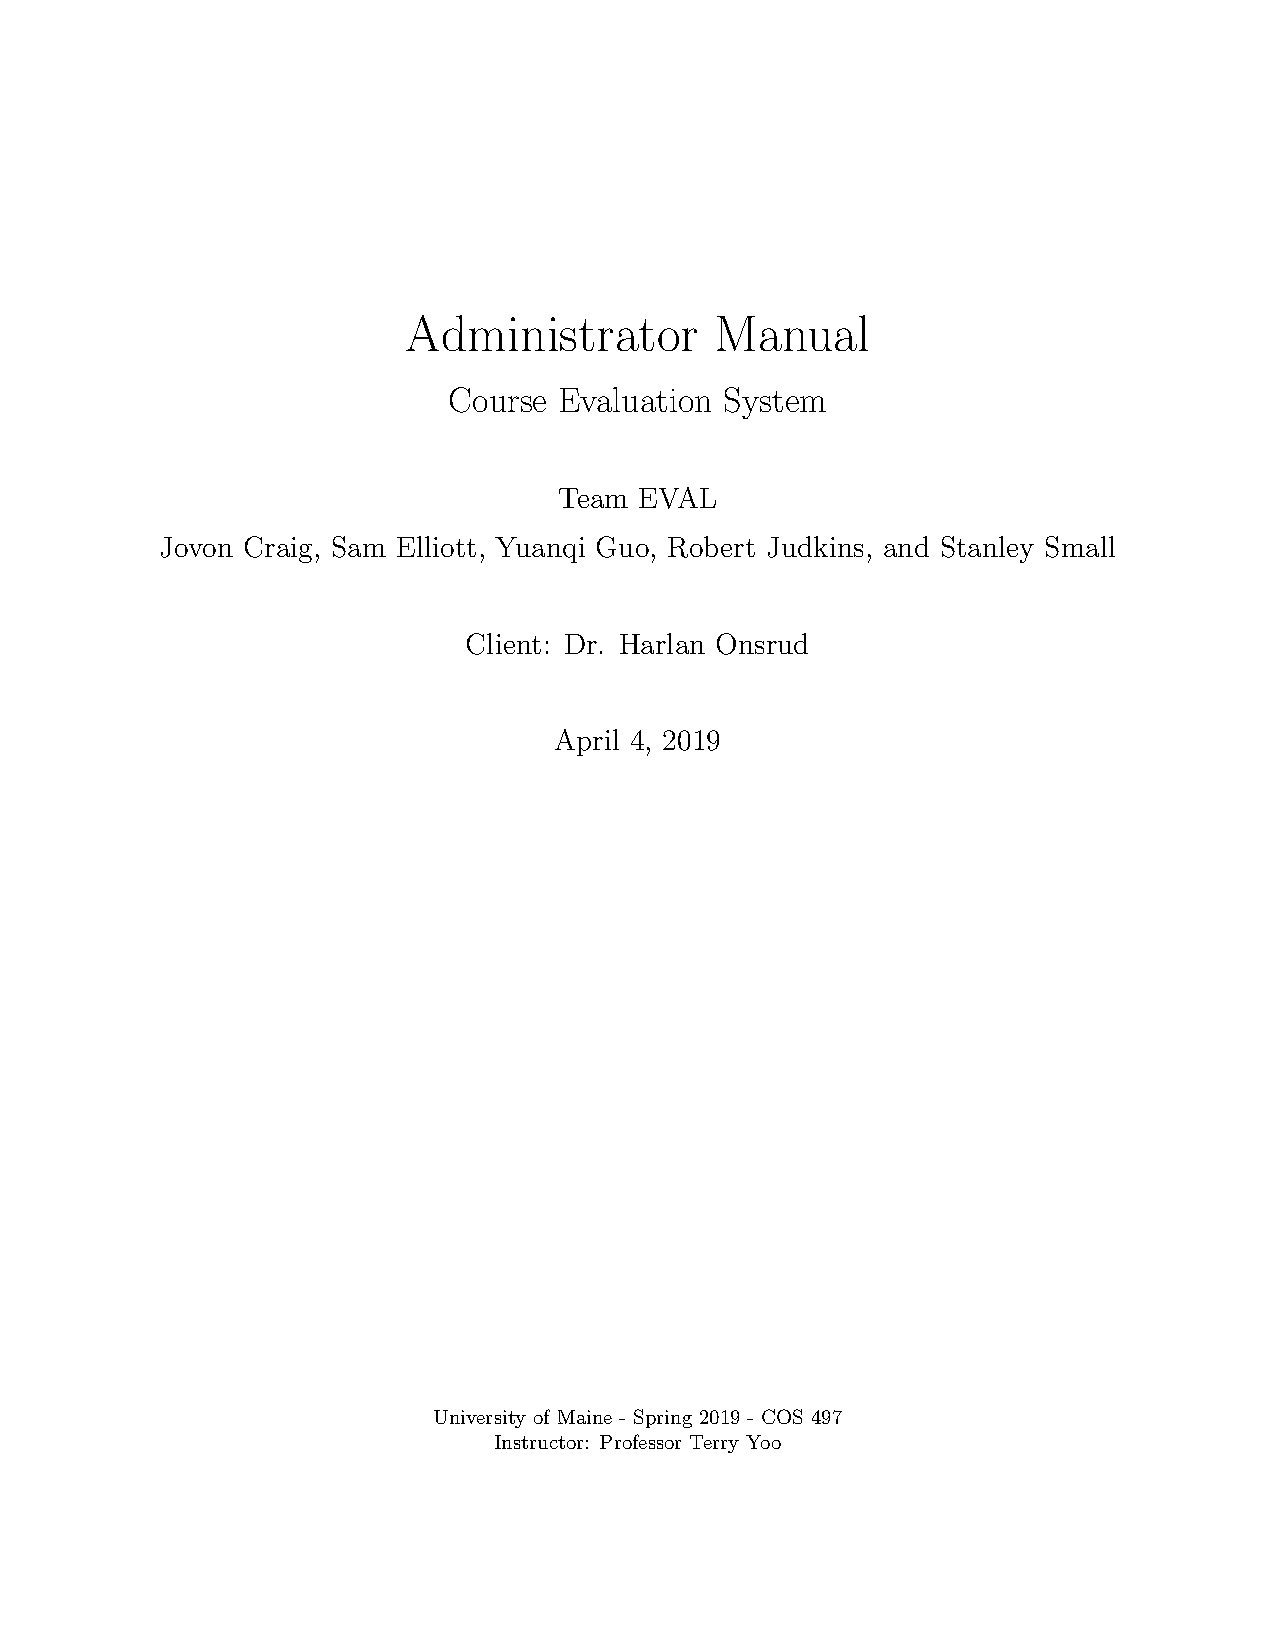
\includepdf[scale=0.85,pages=1,pagecommand=\section{Administrator Manual}]{am.pdf}
\includepdf[scale=0.85,pages=2-]{am.pdf}

\newpage

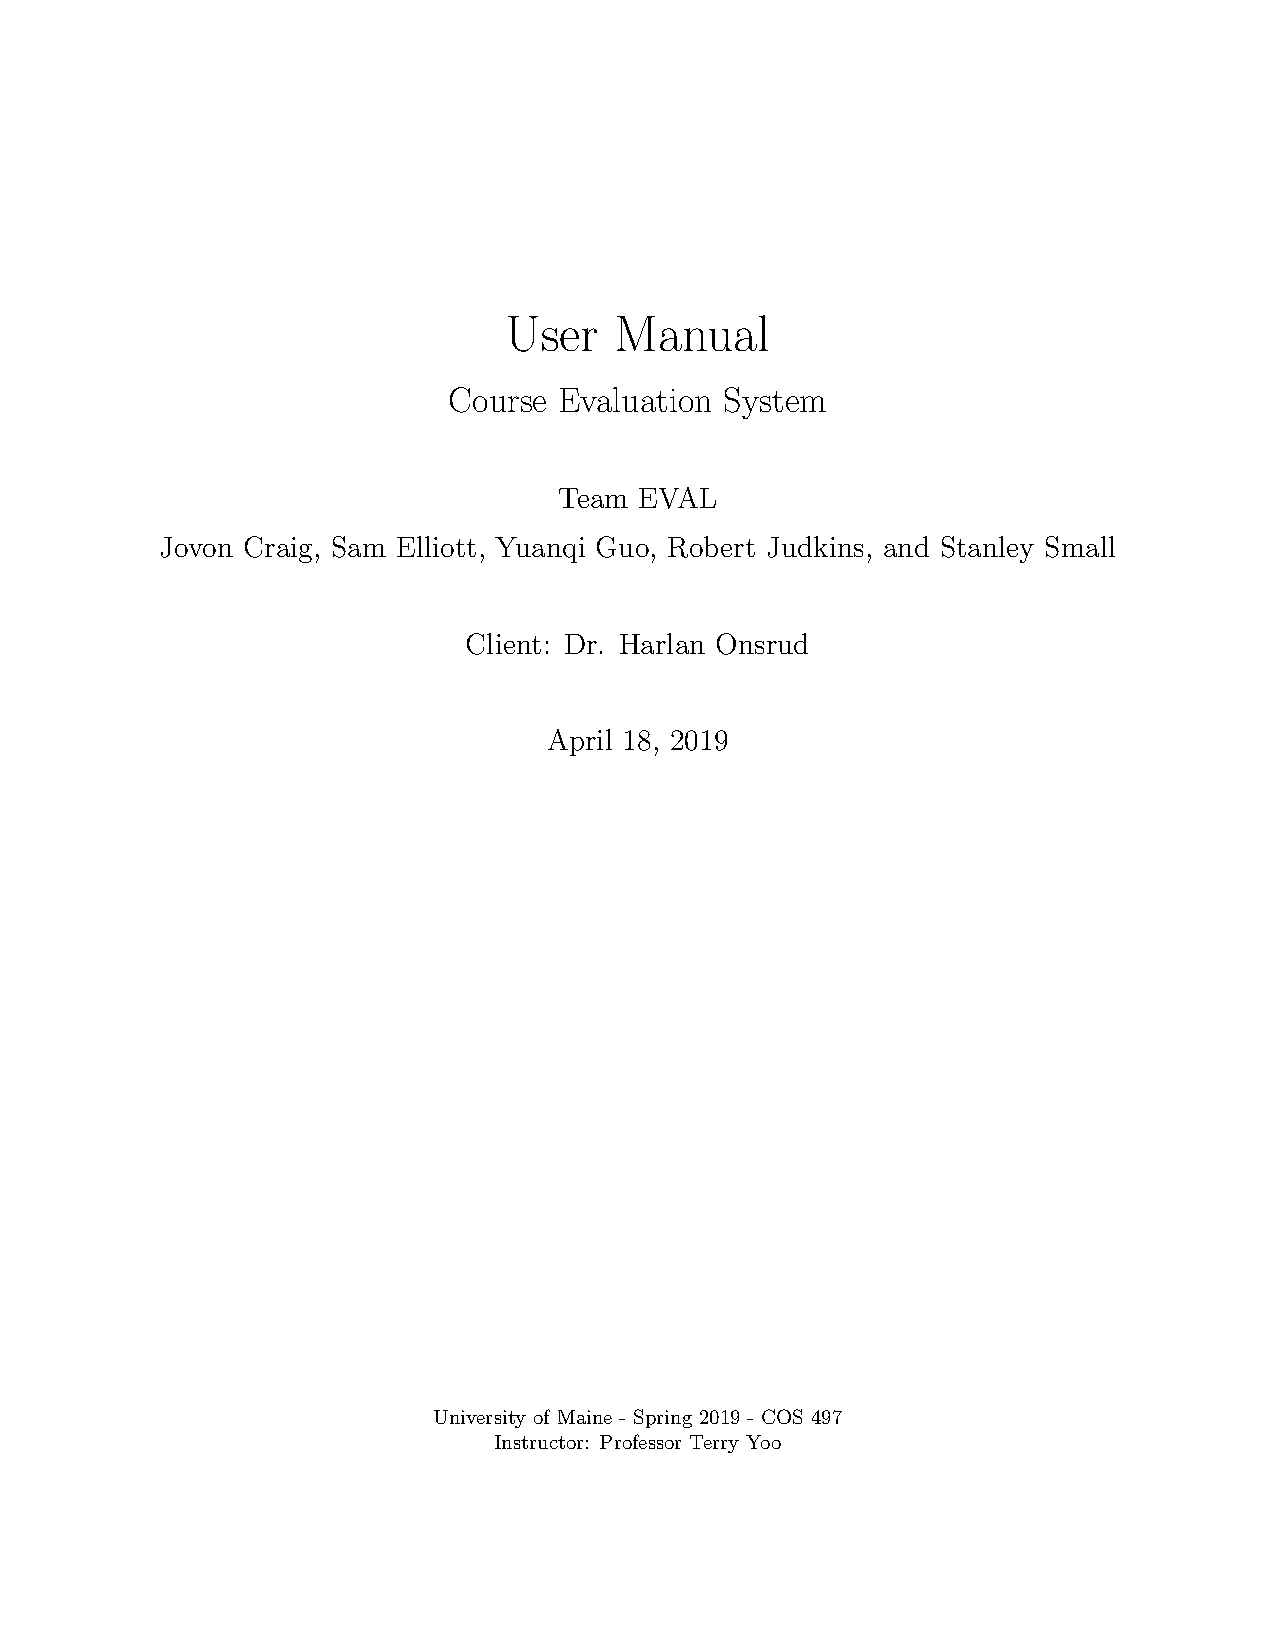
\includepdf[scale=0.85,pages=1,pagecommand=\section{User Manual}]{um.pdf}
\includepdf[scale=0.85,pages=2-]{um.pdf}

\newpage

\includepdf[scale=0.85,pages=1,pagecommand=\section{Example Question Selection Form}]{images/question_appendix.pdf}
\includepdf[scale=0.85,pages=2-]{images/question_appendix.pdf}

\newpage

\includepdf[scale=0.92,pages=1,pagecommand=\section{Example Results Display}]{images/results_appendix.pdf}
\includepdf[scale=0.92,pages=2-]{images/results_appendix.pdf}

\end{document}
